\graphicspath{{lit_study/fig/}}

{
\tikzset{external/figure name/.add={lit_study/}{}}


\chapter{Literature study}
\label{chap:lit_study}

\section{Unknown suspended payloads}

    \paragraph
    Figure~\ref{fig:real_suspended_payload_example} shows an example of a practical use case of a multirotor with a suspended payload.
    Items are placed in a water proof bag and transported by the multirotor to a place of need.
    Note that the multirotor does not know the dynamics of the payload before flight, 
    because the items may change depending on the need in the specific situation. 
    The shape and mass of the loaded items will have an effect on swing of the payload, 
    and the control system should be able to fly well despite the altered flight dynamics.

    \begin{figure}[htb]
        \centering
        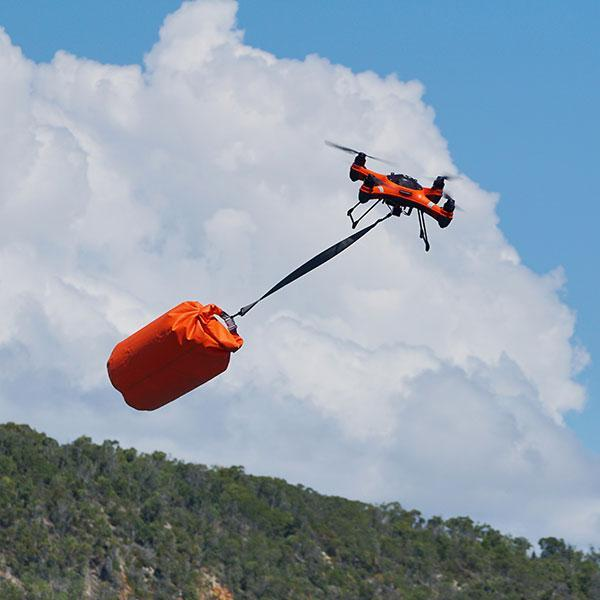
\includegraphics[width=0.45\linewidth]{real_suspended_payload_example.jpg}            
        \caption{A practical suspended payload used for search and rescue missions \cite{CompareCommander2020}}
        \label{fig:real_suspended_payload_example}
    \end{figure}

    % Active vs passive attachments
    % https://hybrid-robotics.berkeley.edu/publications/ACC2017_QuadLoad_ElasticCable.pdf
    % In terms of mechanical design, several methods have been
    % proposed to attach a payload to a UAV, involving both active
    % and passive attachments. Examples of active attachments
    % include using actuated grippers to grip and pickup payloads
    % [13], [10], and actuated manipulator arms to enable aerial
    % manipulation [10]. These active mechanisms provide more
    % degrees-of-freedom (DOFs) to the UAV, and help in active
    % aerial manipulation. However, these advantages come at
    % the cost of loss of agility of the small UAVs due to the
    % added inertia to the system. Moreover, actuated gripper arms
    % introduce dynamic coupling between the manipulator and
    % quadrotor which needs to be accurately captured in the
    % mathematical model and compensated by the controller.
    % Passive type of attachments have also been developed,
    % wherein the payload is attached to the UAVs through a mechanical cable or tether [2], [15], [17], [6], [18]. By attaching
    % the payload through tethers, the payload could be connected
    % to a single or multiple UAVs without directly modifying the
    % UAV’s inertia. However, this becomes more challenging for
    % control due to the additional degree-of-underactuation. Early
    % work looked at the transportation of a single point-mass load
    % 1P. Kotaru, G. Wu are with Department of Mechanical Engineering,
    % Carnegie Mellon University, 5000 Forbes Avenue, Pittsburgh PA, 15213,
    % email: {vkotaru,gwu}@andrew.cmu.edu.
    % K. Sreenath is with the Depts. of Mechanical Engineering, The Robotics
    % Institute, and Electrical and Computer Engineering, Carnegie Mellon University, Pittsburgh, PA 15213, email: koushils@cmu.edu.
    % This work is supported in part by the Google Faculty Research Award
    % and in part by NSF grants CMMI-1538869, IIS-1464337, IIS-1526515.
    % Fig. 1: Quadrotor with load through a suspended cable, with
    % the cable modeled as a spring-damper. The configuration
    % space of the system is given as R
    % 3 × SO(3) × S
    % 2 × R,
    % with 9 degrees-of-freedom and 4 actuators, resulting in 5
    % degrees-of-underactuation.
    % with single and multiple helicopters [2], with the objective
    % being to actively cancel any swing in the cable. Furthermore,
    % dynamic programming (DP) based methods were employed
    % to plan dynamically-feasible trajectories that minimized the
    % load swing along with an adaptive controller in [15].

\section{System Identification}
\section{Control systems}

    
    % ?? Lit study: include different types of \gls{MPC}, e.g. DMC, MAC
    % ?? different types of models \cite{}, 
    % ?? See \cite{Garcia1989} for good example of different implementations with different models
    
\section{System Design}
Blok diagram
komponente

}


